\documentclass{unswmaths}
\usepackage{unswshortcuts}
\begin{document}
\author{Adam J. Gray}
\title{Assignment 2}
\subject{Ergodic Theory}
\studentno{3329798}

\unswtitle

\section{}
\subsection{}
\begin{align*}
    T(\theta, \nu) = (\theta + \nu \mod 2\pi, \alpha\nu + \gamma \cos(\theta + \nu))
\end{align*}
\subsection{}
\begin{align*}
    J[T](\theta, \nu) = \left( 
    \begin{array}{cc}
        1   & 1 \\
        -\gamma \sin(\theta + \nu) & \alpha - \gamma\sin(\theta + \nu)
    \end{array}
    \right)
\end{align*}
and so
\begin{align*}
|J[T](\theta, \nu)| &= \alpha - \gamma\sin(\theta + \nu) + \gamma\sin(\theta + \nu) \\
    &= \alpha.
\end{align*}
So $ |J[T](\theta, \nu)| = 0 $ iff $ \alpha = 0 $. So since we have chosen $ \alpha > 0 $ this map is invertible everywhere by the inverse function theorem.
\subsection{}
\begin{figure}[h]
    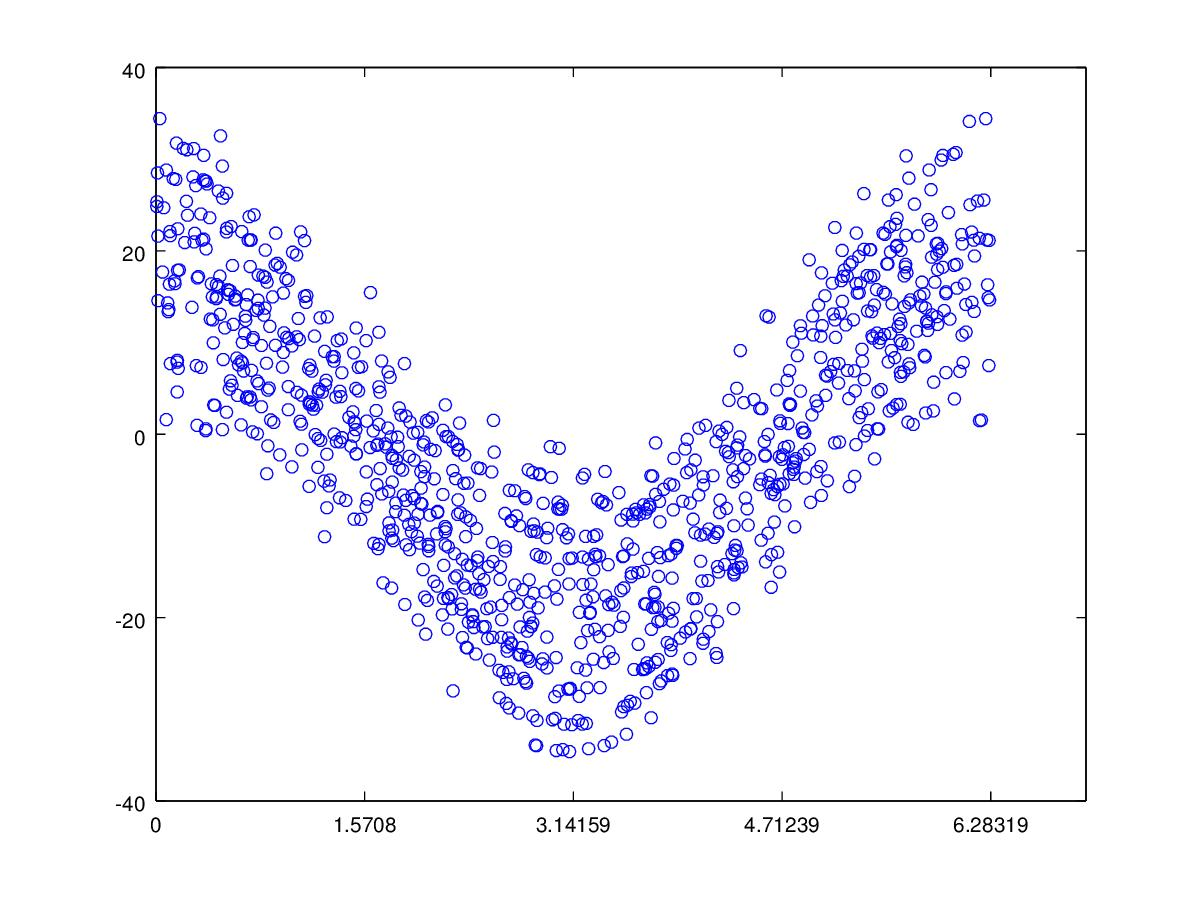
\includegraphics[scale=0.5]{Question_3}
    \caption{Phase plot of velocity vs table phase with $ \theta_0 = 0.5, \nu_0 = 0.5 $}
\end{figure}
\subsection{}
The maximum post-bounce velocities occur near $ \theta = 0 $ ($\theta = 2\pi$). This makes sense because the piston is traveling in the opposite direction to the ball. This is happening fastest at $ \theta = 0 $ and so this results in the largest bounces. The minimum is found at $ \theta = \pi $. This also makes sense because this is when the piston is traveling in the same direction as the ball. This is happening fastest at $ \theta = \pi $ and this results in the largest slowdown in the bounce.

\subsection{}
\subsection{}
\label{qn_6_ergodic}
\begin{figure}[h]
    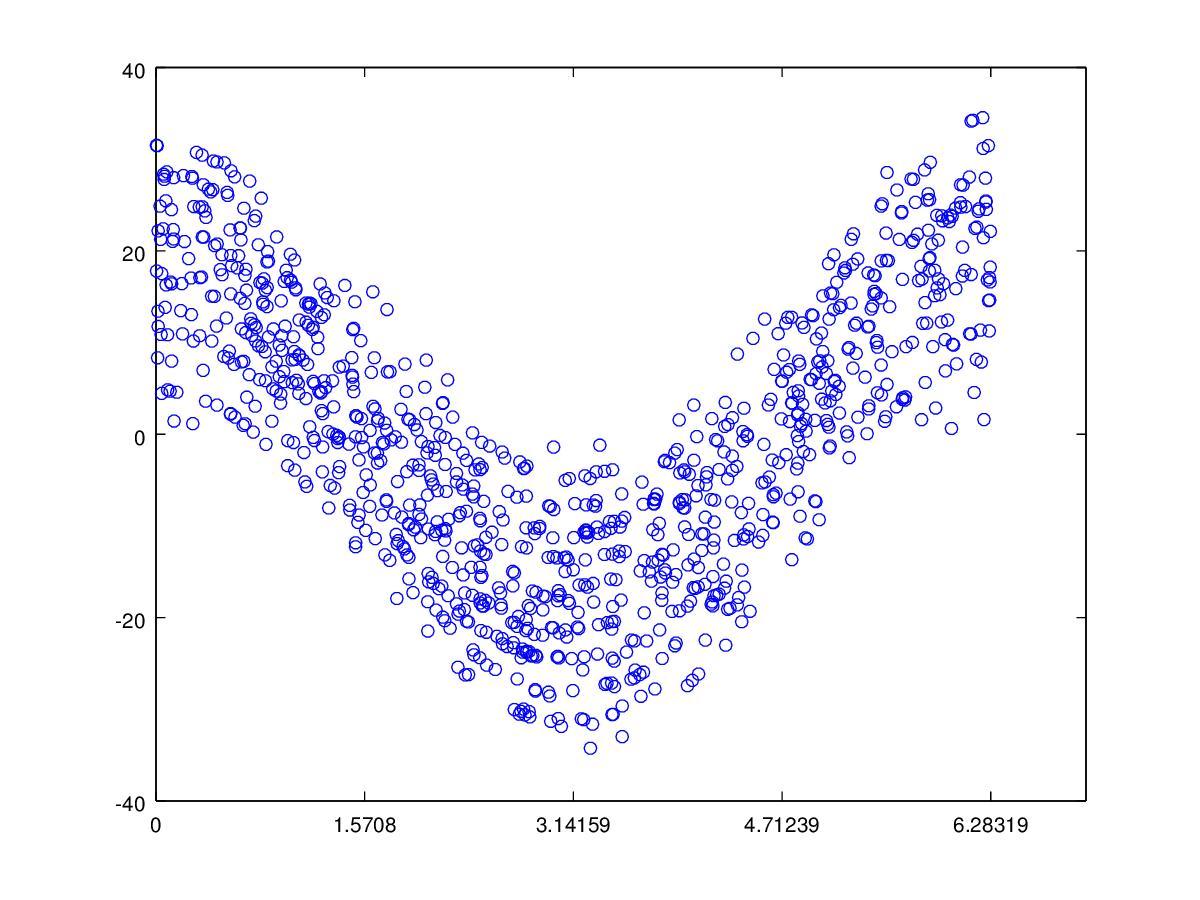
\includegraphics[scale=0.5]{Question_6_Ergodic}
    \caption{A bundle of 1000 points starting near $ \theta_0 = 0.5,  \nu_0 = 0.5 $ were iterated through $  T $ 10000 times}
\end{figure}

What figure 2 shows is that a small ball of points \emph{spreads out} in the phase space. Note that this ensemble of points roughly matches the orbit of one point. This would lead us to suspect that this process is Ergodic. 

\clearpage
\begin{figure}[h]
    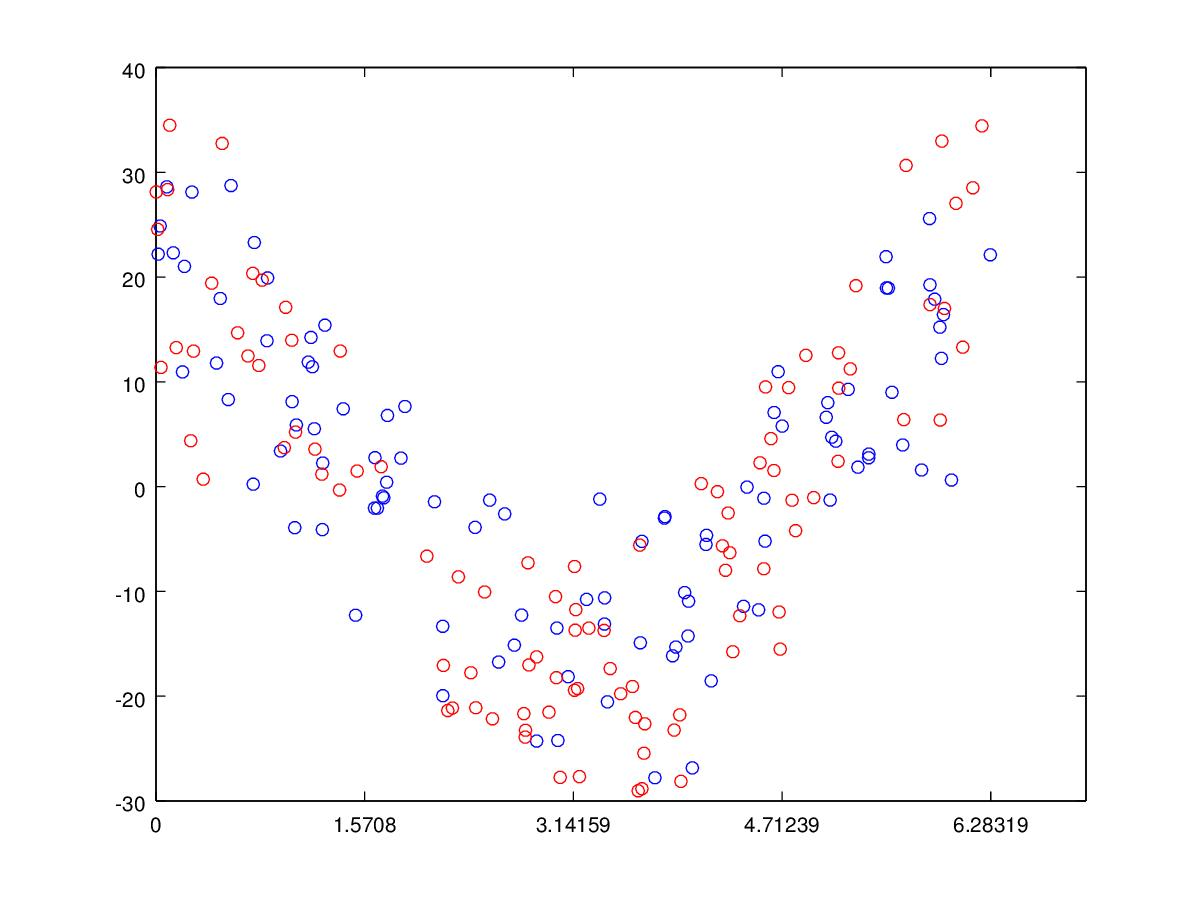
\includegraphics[scale=0.5]{Question_6_Mixing}
    \label{qn_6_mixing}
    \caption{Two bundles of 200 points after iterating through  $ T $ 10000 times. Blue started near $ \theta_0 = 0.5, \nu_0 = 0.5 $ while red started near $ \theta_0 = 1, \nu_0 = 1 $ }
\end{figure}


Figure 3 suggests that the long term behaviour of the  points is independent of their starting point. That is two sets of balls mix together. Although only testing with two bundles of balls is hardly rigerous, even empirically, this would suggest that this process is mixing.
\subsection{}
Since we suspect that this process is Ergodic (and mixing) this question can be answered by watching the long term behavior of 1 point. We do this for a point starting at $ \theta_0 = 0.5, \nu_0 = 0.5 $ and see that $ 49.95 \% $ of the first 10000 bounces occur when $ \theta < \pi / 2 $ or $ \theta > 3\pi / 2 $, that is when the piston is moving up. We conclude that there is equal chance of the ball hitting on a down stroke compared to an upstroke.

\subsection{}
Again since we suspect that this process is Ergodic we just study the evolution of one point.

\end{document}




